\documentclass{article}

\usepackage[utf8]{inputenc}
\usepackage[T1]{fontenc}
\usepackage[francais]{babel}
\usepackage{titling}
\setlength{\droptitle}{-3cm}
\usepackage{graphicx} 

\title{Définition de la question de recherche et mise en place des outils de travail collaboratif}
\author{CAROT Axel, ARISOY Ivan Can, \\ DARDE Guilhem, NDJINGA NDJINGA Anta Claude}
\date{\today}

\begin{document}
\maketitle

\section{Mise en place des outils de travail collaboratif}

Dans un premier temps, nous avons mis en place les outils de travail collaboratif qui joueront un rôle central dans le bon déroulement de notre projet.

\subsection{Github}
Nous avons créé un dépôt privé sur la plateforme GitHub qui regroupe l'ensemble de notre travail.Il comprend divers éléments essentiels :
\begin{itemize}
    \item \textbf{Un fichier README.md} qui présente de manière concise le nom du projet choisi, une brève description de notre sujet, une liste complète des membres du groupe avec leurs adresses e-mail UPV, ainsi que des liens vers nos divers outils collaboratifs.
    \item \textbf{Différents dossiers} organisés en fonction de leur contenu, notamment l'AgendaMinutes pour les comptes rendus de nos réunions, la Bibliographie, les Données brutes, les Codes source, les Rapports, et les Soutenances prévues.
\end{itemize}

\subsection{Discord}
Pour faciliter la communication et la gestion de notre projet, nous avons créé un serveur Discord dédié. Ce serveur est structuré en plusieurs sections :
\vspace{0.2cm}

\begin{minipage}{0.7\textwidth}
\begin{itemize}
    \item \textbf{Général} pour les discussions générales et les échanges d'idées.
    \item \textbf{Planification de sessions} pour l'organisations de nos sessions de travail.
    \item \textbf{Biblio et ressources} pour partager et discuter des ressources bibliographiques pertinentes pour notre recherche.
    \item \textbf{Deadlines} Cette section est dédiée au suivi de nos dates butoirs.\\
\end{itemize}
\end{minipage}
\vspace{-0.5cm}
\begin{minipage}{0.2\textwidth}
  \centering
  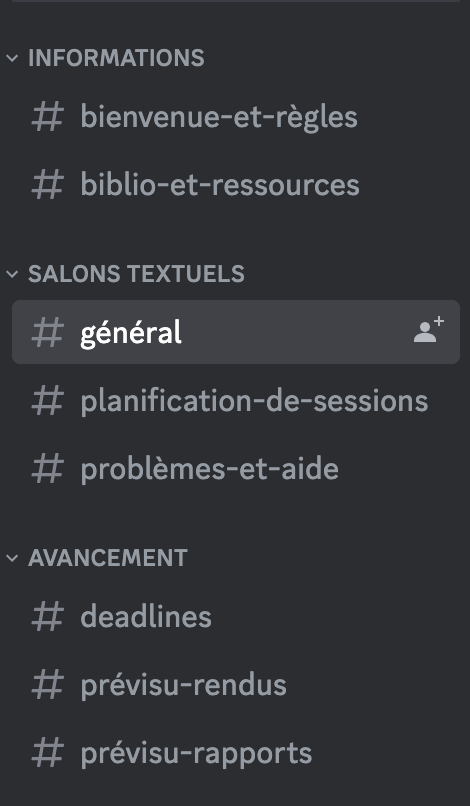
\includegraphics[width=\linewidth]{discord.png}
  \label{fig:label}
\end{minipage}

\vspace{1.0 cm}
Toutes ces rubriques contribuent à une transmission fluide des informations au sein de l'équipe.

\subsection{Trello}
Notre organisation actuelle repose principalement sur la répartition des tâches en vue des échéances liées aux rapports à rendre au cours du semestre. Trello nous permet d'avoir des visualisations graphiques pour une meilleure représentation visuelle de notre planification. 

\begin{figure}[h]
    \centering
    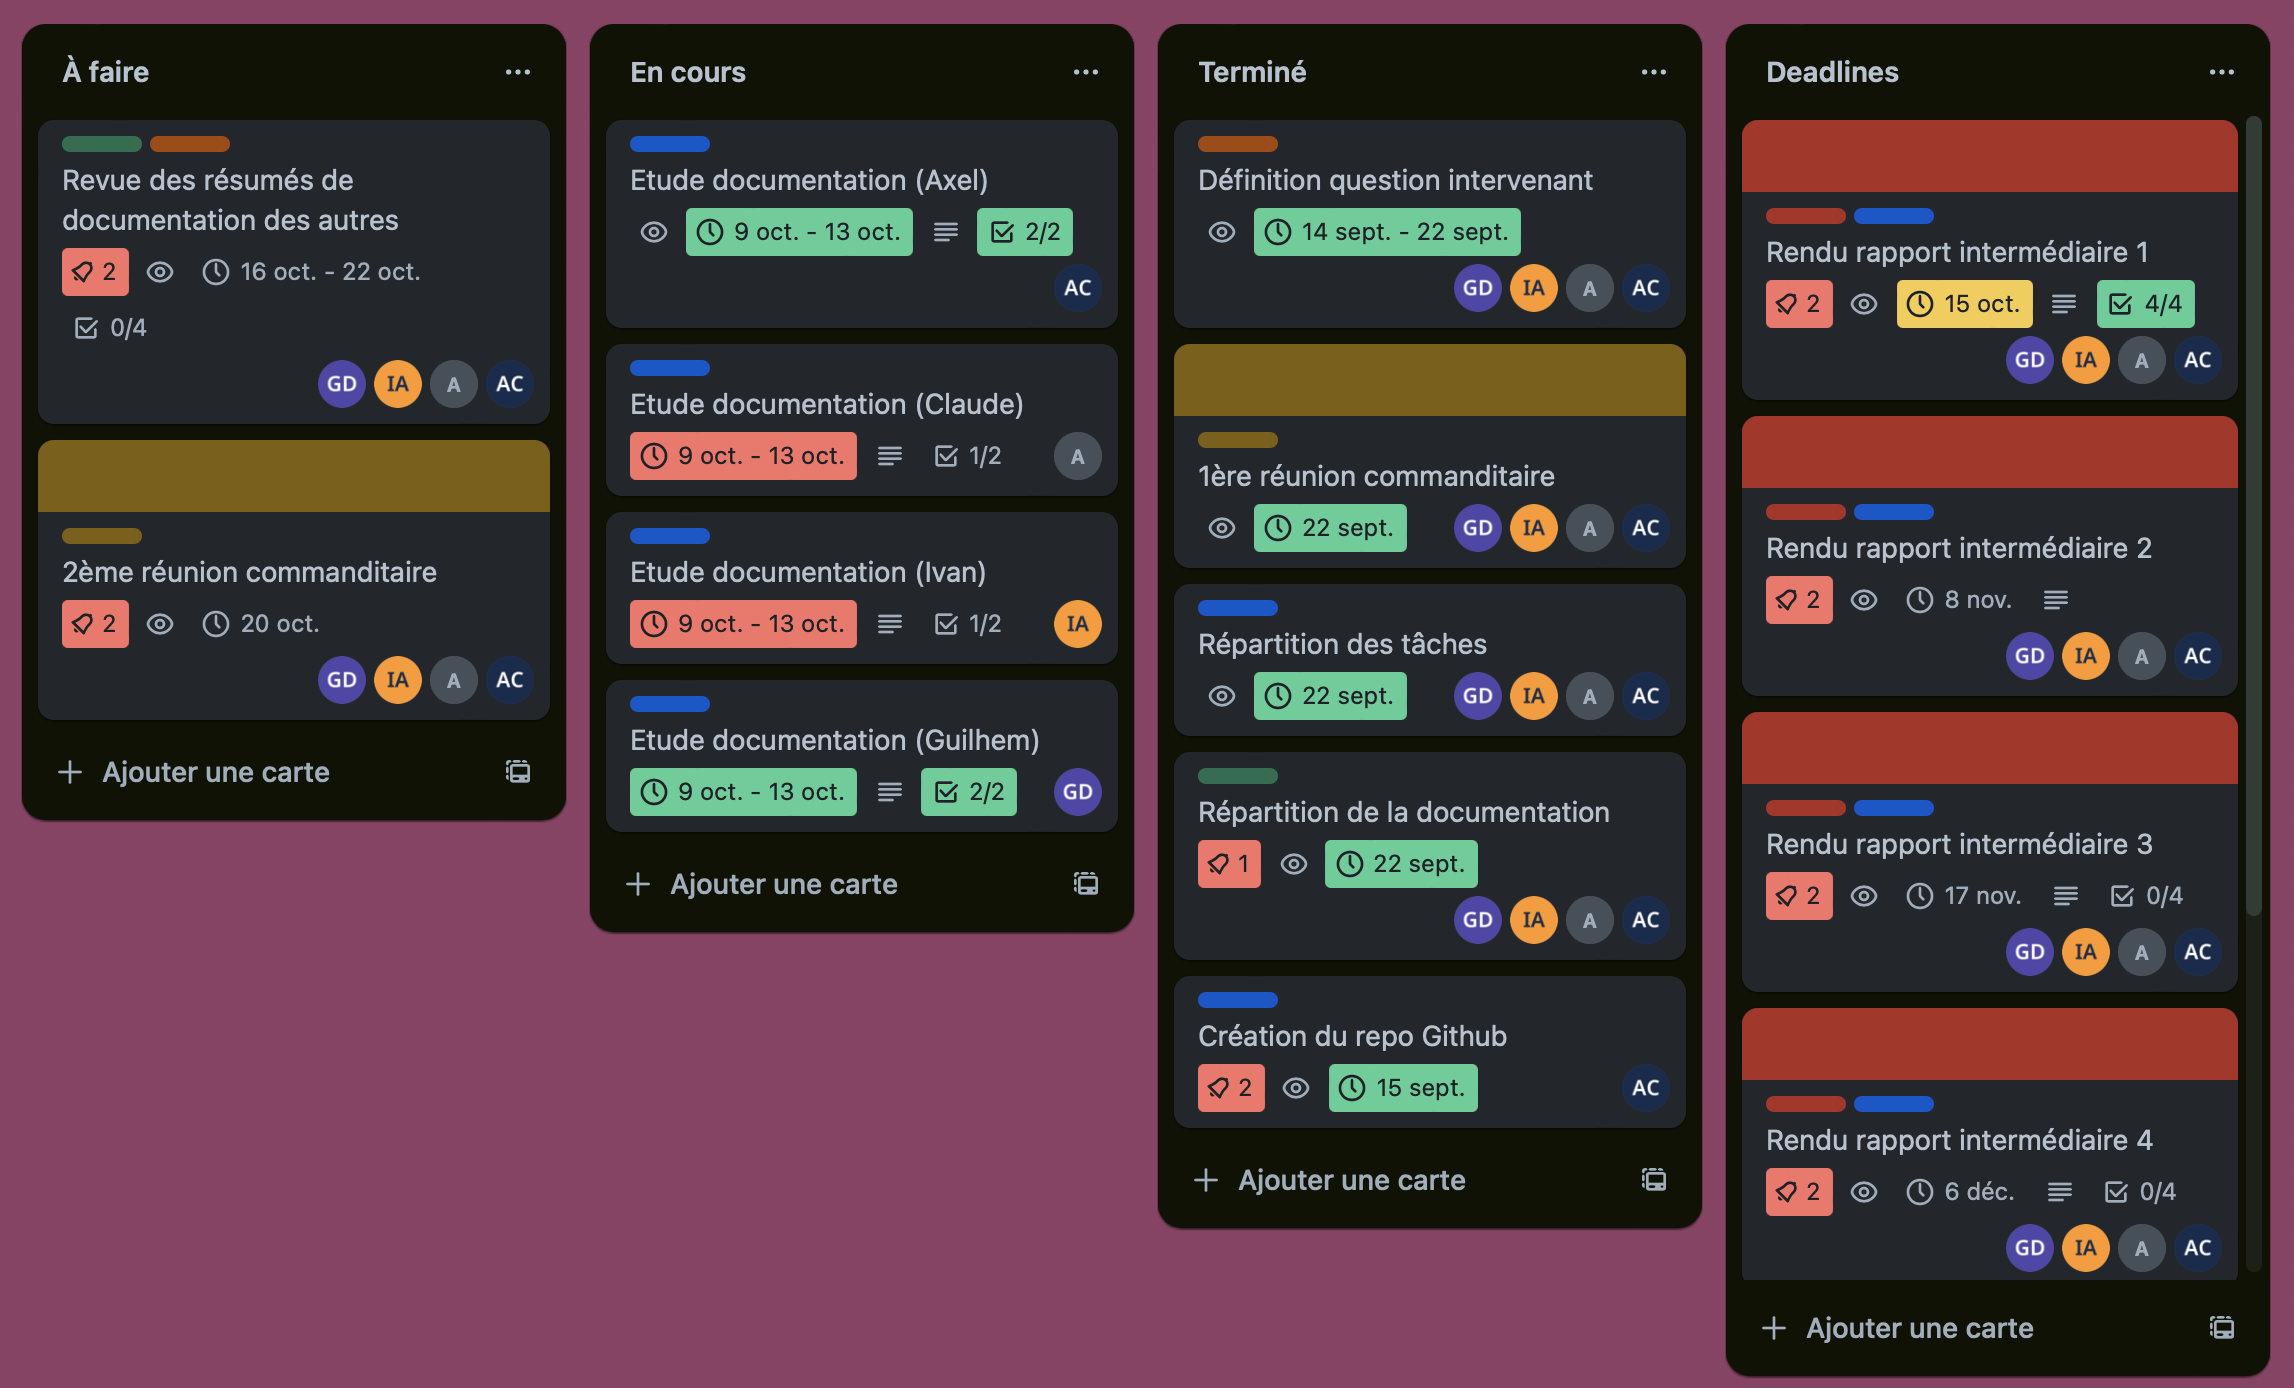
\includegraphics[width=0.8\textwidth]{trello.png}
    \caption{Trello}
    \label{fig:mon_image}
\end{figure}

\subsection{Google Agenda}
L'utilisation de Google Agenda nous permet de synchroniser nos rendez-vous, de fixer les dates de nos débriefings et de suivre nos diverses échéances. 

\section{Définition de la question de recherche}

\subsection{Premier rendez-vous avec les commanditaires}
Après avoir mis en place les outils collaboratifs, nous avons pris un premier rendez-vous avec nos commanditaires pour leur poser toutes nos questions que nous avions préparées préalablement en relation avec notre sujet de recherche.\\

Nous avons fait l'entretien avec Roberto INTERDONATO et Sarah VALENTIN, deux chercheurs du CIRAD, qui est un organisme français spécialisé dans la recherche agronomique et la coopération internationale en faveur du développement durable des régions tropicales et méditerranéennes. Cette rencontre initiale a été fondamentale pour établir une compréhension commune de nos objectifs, de la portée de notre projet, et des attentes de nos commanditaires.

\subsection{Les données}
Les données textuelles ont été collectées au fil des deux dernières années à travers des techniques de web scraping. Elles proviennent de diverses sources, notamment des journaux locaux, totalisant plus de 20 000 articles, de transcriptions de vidéos YouTube, ainsi que de podcasts abordant les actualités des différents pays de l'Afrique de l'Ouest (avec un focus sur le Burkina Faso, le Bénin et le Sénégal). Ces données ne se limitent pas uniquement à des informations récentes, car elles intègrent également des sources d'informations plus anciennes. Elles nous ont été transmises dans un dossier partagé via WeTransfer.

\subsection{La documentation}
Les commanditaires nous ont fourni une documentation composée de :
\begin{itemize}
    \item Différents articles portant sur la sécurité alimentaire.
    \item Un notebook d'analyse descriptive et des lexiques.
    \item Une liste de bibliothèques Python à utiliser (NLTK, Spacy, Transformers).
\end{itemize}

\subsection{Compréhension de la question de recherche}
La réunion en présence des commanditaires nous a permis d'éclaircir notre compréhension de la question de recherche.\\

Premièrement, nous avons fait valider notre reformulation non technique de la problématique. En substance, notre mission consiste à explorer les données textuelles qui, pour diverses raisons, n'ont pas encore été pleinement exploitées par les gouvernements, en particulier en ce qui concerne la sécurité alimentaire en Afrique de l'Ouest. Cette région est confrontée à des défis notables, tels qu'une croissance démographique soutenue, une agriculture fortement tributaire des conditions pluviométriques, et des préoccupations liées à la sécurité et à la santé.

\subsection{Enjeux, défis et attentes}
Les problèmes et enjeux liés à cette recherche résident principalement dans le fait que le CIRAD a une approche pluridisciplinaire et n'est pas spécialisé en statistique. Notre travail permettrait de compléter les visions existantes et de contribuer à une meilleure compréhension des dynamiques complexes qui caractérisent la sécurité alimentaire dans cette région.\\

Le défi central auquel nous devons faire face réside dans la nature non structurée des données textuelles en français, notamment en raison des retranscriptions de vidéos et de podcasts. Cette absence de structure et la présence limitée de ponctuation introduisent un certain niveau de bruit dans nos données. Il nous faudra identifier les articles pertinents liés à la sécurité alimentaire.\\

Les principales tendances ou informations clés que l'on espère découvrir en effectuant une analyse exploratoire des données textuelles sont les événements ponctuels qui ont un impact significatif sur la durée et l'évolution des prix alimentaires. Par exemple, des événements tels que les sécheresses ou les inondations peuvent avoir des répercussions substantielles sur les prix des denrées alimentaires. Notre analyse vise à mettre en lumière ces tendances et à les étayer avec des exemples concrets, tels que les variations de prix du blé.

\section{Stratégies et réalisations}
Nous avons établi les grandes étapes de notre projet avec les commanditaires afin de garantir la progression méthodique de notre recherche :
\begin{itemize}
    \item \textbf{Étiquetage et annotation des données.} Cette tâche essentielle permettra de marquer les éléments clés dans les textes, facilitant ainsi leur compréhension et leur traitement ultérieur.
    \item \textbf{Analyse descriptive.} Cette démarche vise à dégager les tendances et les caractéristiques de nos corpus textuels, ce qui contribuera à une compréhension plus profonde de nos sources.
    \item \textbf{Extraction d'entités nommées.} Cette étape nous permettra d'identifier et d'extraire des informations clés telles que les noms de lieux, de personnes et d'événements, ce qui renforcera notre analyse.
    \item \textbf{Analyse structurelle.} Cette tâche consiste à explorer les relations et les connexions entre les éléments de nos données textuelles. Cette démarche contribuera à établir une vision plus globale des informations à notre disposition.\\
\end{itemize}

Nous avons convenu d'effectuer un rendez-vous environ toutes les deux semaines en fonction de nos avancées. Les commanditaires ont tout de même insisté sur l'importance de les solliciter par mail si nous rencontrons des difficultés.\\

Nous nous sommes répartis la documentation dans l'objectif d'en faire des comptes rendus. Cette démarche renforce notre compréhension collective des ressources. Nous commencerons notre exploration des données par la création de visualisations significatives pour illustrer les résultats de notre analyse exploratoire. Parmi ces visualisations, nous envisageons l'utilisation de Wordclouds, de radar plots et de cartographies pour mettre en évidence les motifs et les tendances les plus pertinents. Nos commanditaires nous ont recommandé l'utilisation de D3.js comme logiciel de data visualization.\\

En ce qui concerne les critères d'évaluation de la qualité et de la précision de nos informations extraites et enrichies, nous mettrons l'accent sur les catégories et les entités nommées telles que les dates, les lieux et les événements en tant que variables clés. Les indicateurs de rappel et de précision constitueront un point d'attention majeur dans notre analyse (des termes que nous devrons approfondir grâce à la bibliographie).

\section{Les erreurs à ne pas commettre}
Nos commanditaires ont souligné certaines erreurs à éviter dans le cadre de notre recherche. L'une de ces erreurs, que nous avons pleinement intégrée, concerne la nécessité d'accorder une attention particulière à la phase préliminaire de notre projet et au nettoyage de nos données.\\

En effet, les données dont nous disposons, comportent des perturbations indésirables que l'on peut qualifier de "bruit". Il est impératif de ne pas sous-estimer ces perturbations, car elles peuvent influencer considérablement la validité de nos résultats. Par conséquent, les chercheurs nous ont déconseillé d'effectuer de la prédiction.\\

En plus de ce facteur, il nous faudra faire attention au contexte d'utilisation des mots dans nos données. Le sens des mots peut être influencé par le contexte, ce qui peut avoir un impact significatif sur l'interprétation des données. 

\end{document}
